
\section{Redes Neuronales Convolucionales (CNN) en Procesamiento del Lenguaje Natural (PLN)}

Las redes neuronales convolucionales (CNN) se volvieron muy populares en la comunidad de visión por computadora debido a su éxito en la detección de objetos ("gato", "bicicletas") independientemente de su posición en la imagen. Estas redes identifican predictores locales indicativos en una estructura (por ejemplo, imágenes, oraciones) y los combinan para producir una representación vectorial de tamaño fijo para la estructura. En el procesamiento del lenguaje natural, la CNN captura los n-gramos que son más informativos para la tarea predictiva objetivo. Por ejemplo, en la clasificación de sentimientos, estos aspectos locales corresponden a n-gramos que transmiten sentimiento, como "no está mal" o "muy bueno". La idea fundamental de las CNN \cite{lecun1998gradient} es considerar la extracción de características y la clasificación como una tarea conjuntamente entrenada.

\section{Convolución Básica + Agrupamiento}

En el procesamiento del lenguaje natural, las oraciones suelen ser modeladas como secuencias de vectores de palabras. Estos vectores se pueden obtener a partir de incrustaciones de palabras pre-entrenadas o de una capa de incrustación. La CNN aplica funciones no lineales (aprendidas) o "filtros" que mapean ventanas de tamaño $k$ de palabras a valores escalares. Se pueden aplicar varios filtros, lo que resulta en un vector de dimensión $l$ (una dimensión por filtro). Los filtros capturan propiedades relevantes de las palabras en la ventana y corresponden a la "capa de convolución" de la red. La capa de "agrupamiento" se utiliza para combinar los vectores resultantes de las diferentes ventanas en un solo vector de dimensión $l$. Esto se logra tomando el valor máximo o el valor promedio observado en cada dimensión en las diferentes ventanas. El objetivo es capturar las características más importantes de la oración, independientemente de la posición. El vector resultante de dimensión $l$ se alimenta luego a una red que se utiliza para la predicción (por ejemplo, softmax). Los gradientes se propagan desde la pérdida de la red ajustando los parámetros del filtro. Los filtros aprenden a resaltar los aspectos de los datos (n-gramos) que son importantes para la tarea objetivo.

\begin{figure}[h]
  \centering
  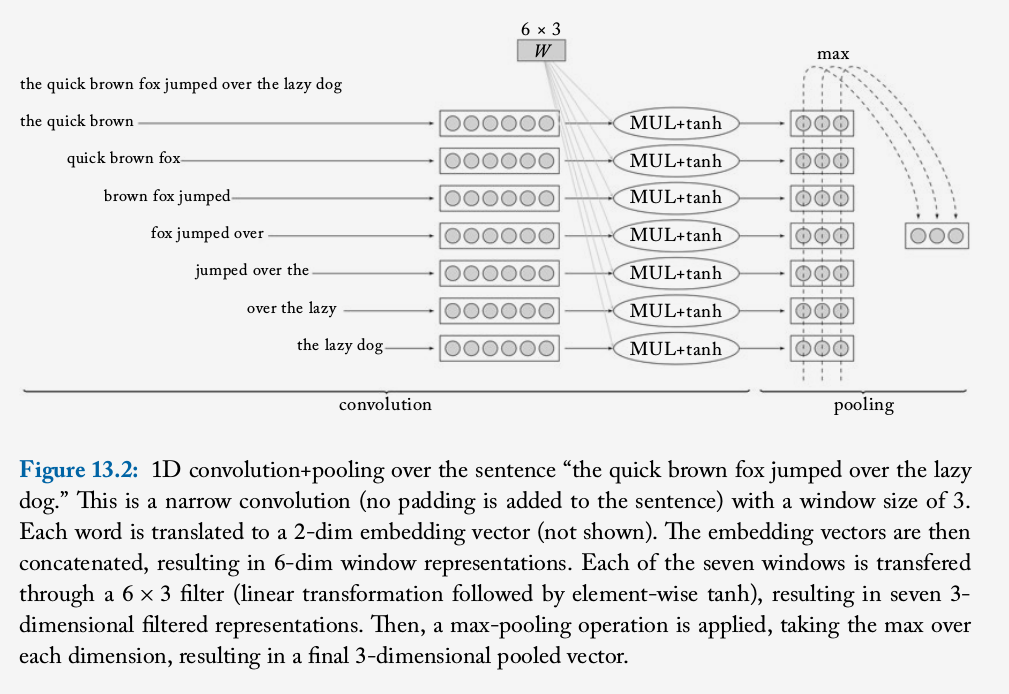
\includegraphics[scale=0.28]{pics/CNN.png}
  \caption{Arquitectura básica de una CNN para procesamiento del lenguaje natural.}
  \label{fig:cnn}
  \footnotemark{Fuente: \cite{goldberg2017neural}}
\end{figure}

\section{Convoluciones 1D sobre Texto}

En el contexto del procesamiento del lenguaje natural, nos centramos en la operación de convolución unidimensional\footnote{1D se refiere a una convolución que se aplica a entradas unidimensionales como secuencias, a diferencia de las convoluciones 2D que se aplican a imágenes.}. Consideremos una secuencia de palabras $w_{1:n} = w_1, \dots, w_n$, cada una con su vector de palabras de $d_{emb}$ dimensiones correspondiente $E_{[w_i]} = \vec{w}_{i}$. Una convolución 1D de ancho $k$ funciona deslizando una ventana de tamaño $k$ sobre la oración y aplicando el mismo filtro a cada ventana en la secuencia. Un filtro es un producto escalar con un vector de pesos $\vec{u}$, seguido a menudo de una función de activación no lineal. Definimos el operador $\oplus (w_{i:i+k-1})$ como la concatenación de los vectores $\vec{w}_{i}, \dots, \vec{w}_{i+k-1}$. El vector concatenado de la ventana $i$-ésima es $\vec{x}_{i} = \oplus (w_{i:i+k-1}) = [\vec{w}_{i};\vec{w}_{i+1};\dots;\vec{w}_{i+k-1}]$, donde $x_{i} \in \mathbb{R}^{k \cdot d_{emb}}$. Luego, aplicamos el filtro a cada vector de ventana, lo que resulta en valores escalares $p_{i} = g(\vec{x}_{i} \cdot \vec{u})$, donde $p_{i} \in \mathbb{R}$. Es común usar $l$ filtros diferentes $\vec{u}_1, \dots, \vec{u}_l$, que se pueden organizar en una matriz $U$, y a menudo se agrega un vector de sesgo $\vec{b}$: $\vec{p}_{i} = g(\vec{x}_{i} \cdot U + \vec{b})$. Cada vector $\vec{p}_i$ es una colección de $l$ valores que representan (o resumen) la $i$-ésima ventana ($\vec{p}_{i} \in \mathbb{R}^l$). Idealmente, cada dimensión captura un tipo diferente de información indicativa. La idea principal detrás de la capa de convolución es aplicar la misma función parametrizada a todos los n-gramos en la secuencia, lo que crea una secuencia de $m$ vectores, cada uno representando un n-gramo particular en la secuencia. La representación es sensible a la identidad y al orden de las palabras dentro del n-gramo, pero se extraerá la misma representación para un n-gramo independientemente de su posición en la secuencia.

\section{Convoluciones Angostas vs. Amplias}

¿Cuántos vectores $\vec{p}_i$ tenemos? Para una oración de longitud $n$ con una ventana de tamaño $k$, hay $n - k + 1$ posiciones en las que se puede comenzar la secuencia. Obtenemos $n - k + 1$ vectores $\vec{p}_{1:n-k+1}$. Este enfoque se conoce como \textbf{convolución angosta}. Una alternativa es rellenar la oración con $k - 1$ palabras de relleno a cada lado, lo que resulta en $n + k + 1$ vectores $\vec{p}_{1:n+k+1}$. Esto se llama \textbf{convolución amplia}.

\section{Agrupamiento Vectorial}

Aplicar la convolución sobre el texto da como resultado $m$ vectores $\vec{p}_{1:m}$,

cada uno de los cuales es un vector $\vec{p}_i \in \mathbb{R}^l$. Estos vectores se combinan (se agrupan) en un solo vector $\vec{c} \in \mathbb{R}^l$ que representa toda la secuencia. Existen dos operaciones de agrupamiento comunes:

\begin{itemize}
  \item Max pooling: este operador toma el valor máximo en cada dimensión (es la operación de agrupamiento más común). Para cada dimensión $j$, se calcula $\vec{c}_{[j]} = \max_{1 < i \leq m} \vec{p}_{i[j]}$, donde $\vec{p}_{i[j]}$ denota la $j$-ésima componente de $\vec{p}_i$.

  \item Average pooling: este operador toma el valor promedio en cada índice. Se calcula $\vec{c} = \frac{1}{m} \sum_{i=1}^{m} \vec{p}_i$.
\end{itemize}

Idealmente, el vector $\vec{c}$ capturará la esencia de la información importante en la secuencia. La naturaleza de la información importante que debe ser codificada en el vector $\vec{c}$ depende de la tarea. Por ejemplo, si estamos realizando clasificación de sentimientos, la esencia son los n-gramos informativos que indican sentimiento. Durante el entrenamiento, el vector $\vec{c}$ se alimenta a capas de red adicionales (por ejemplo, una capa de perceptrón multicapa), culminando en una capa de salida que se utiliza para la predicción. El procedimiento de entrenamiento de la red calcula la pérdida con respecto a la tarea de predicción, y los gradientes de error se propagan hacia atrás a través de las capas de agrupamiento y convolución, así como a través de las capas de incrustación. El proceso de entrenamiento ajusta la matriz de convolución $U$, el vector de sesgo $\vec{b}$, la red posterior y potencialmente también la matriz de incrustación $E$\footnote{Algunas personas dejan fija la capa de incrustación durante el entrenamiento, mientras que otros permiten que los parámetros cambien.} de manera que el vector $\vec{c}$ resultante del proceso de convolución y agrupamiento realmente codifique información relevante para la tarea en cuestión.

\section{Clasificación de Sentimientos en Twitter con CNN}

En \cite{Severyn2015} se desarrolla una arquitectura de red neuronal convolucional para la clasificación de sentimientos en Twitter. Cada tweet se representa como una matriz cuyas columnas corresponden a las palabras en el tweet, preservando el orden en el que aparecen. Las palabras se representan mediante vectores densos o incrustaciones entrenadas a partir de un gran corpus de tweets no etiquetados utilizando word2vec. La red está formada por las siguientes capas: una capa de entrada con la matriz de tweets dada, una única capa de convolución, una función de activación lineal rectificada (ReLU), una capa de agrupamiento máximo (max pooling) y una capa de clasificación softmax. Los pesos de la red neuronal se pre-entrenan utilizando datos con anotaciones de emoticonos y luego se entrenan con los tweets anotados a mano del concurso SemEval. Los resultados experimentales muestran que la fase de pre-entrenamiento permite una inicialización adecuada de los pesos de la red y, por lo tanto, tiene un impacto positivo en la precisión de la clasificación.

\begin{figure}[h]
  \centering
  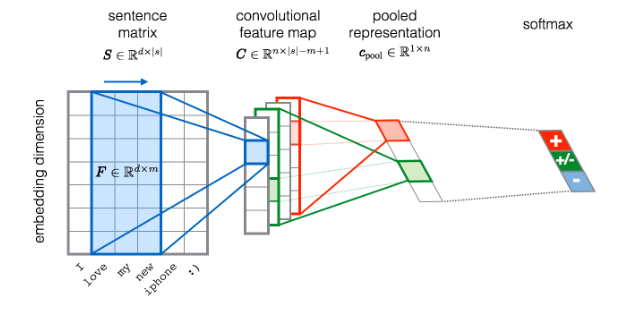
\includegraphics[scale=0.45]{pics/cnn-twitter.png}
  \caption{Arquitectura CNN para la clasificación de sentimientos en Twitter.}
  \label{fig:cnn-twitter}
\end{figure}

\section{Redes Neuronales Convolucionales Muy Profundas para la Clasificación de Texto}

Las arquitecturas de CNN para PLN son bastante superficiales en comparación con las redes neuronales convolucionales profundas que han impulsado el estado del arte en visión por computadora. En \cite{conneau2017very} se propone una arquitectura de red neuronal para el procesamiento de texto (VDCNN) que opera directamente a nivel de caracteres y utiliza solo convoluciones pequeñas y operaciones de agrupamiento. En lugar de utilizar incrustaciones de palabras, se utilizan incrustaciones de nivel de caracteres. Los caracteres son la representación atómica más baja del texto. El rendimiento de este modelo aumenta con la profundidad: utilizando hasta 29 capas de convolución, los autores informan mejoras sobre el estado del arte en varias tareas públicas de clasificación de texto. Las mejoras más notables se logran en conjuntos de datos grandes. Este fue uno de los primeros trabajos que mostró los beneficios de las arquitecturas neuronales profundas para PLN.

\begin{figure}[h]
  \centering
  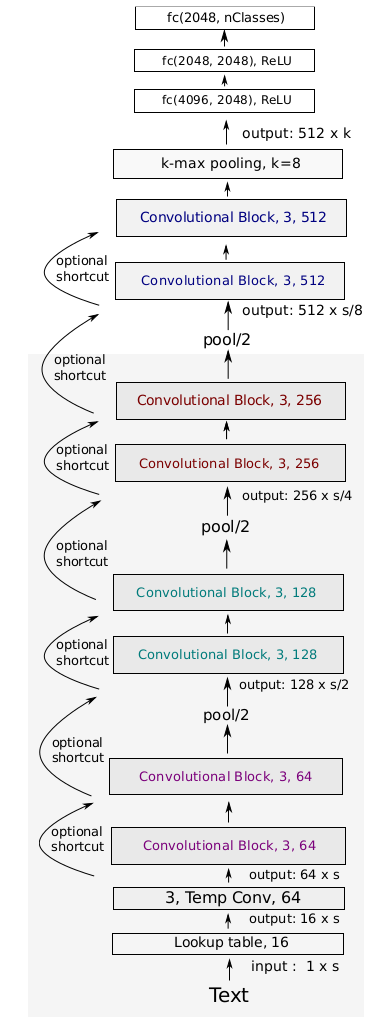
\includegraphics[scale=0.2]{pics/VDCNN.png}
  \caption{Arquitectura VDCNN para la clasificación de texto.}
  \label{fig:vdcnn}
\end{figure}

